% Editable standalone vector figure extracted from novogaia_spectra.tex.
% Source slide 5; figure 04; native embedded fonts.
% Compile with LuaLaTeX from this directory, or run ../export_figures.py.
\documentclass[tikz,border=0pt]{standalone}
% Shared editable preamble for standalone, Nature-style vector figures.
% Text remains embedded and searchable. This is a house-style target, not a
% claim of acceptance or of satisfying every journal's submission checklist.
\usepackage{fontspec}
\setmainfont{LiberationSans}[
  Path=../assets/,Extension=.ttf,
  UprightFont=*-Regular,BoldFont=*-Bold,ItalicFont=*-Italic,BoldItalicFont=*-BoldItalic]
\setsansfont{LiberationSans}[
  Path=../assets/,Extension=.ttf,
  UprightFont=*-Regular,BoldFont=*-Bold,ItalicFont=*-Italic,BoldItalicFont=*-BoldItalic]
\setmonofont{LiberationSans}[
  Path=../assets/,Extension=.ttf,
  UprightFont=*-Regular,BoldFont=*-Bold,ItalicFont=*-Italic,BoldItalicFont=*-BoldItalic]
\usepackage{unicode-math}
\setmathfont{Latin Modern Math}
\DeclareMathSizes{5.9}{6}{5}{5}
\DeclareMathSizes{6}{6}{5}{5}
\usepackage{tikz}
\usetikzlibrary{arrows.meta,calc,positioning,patterns,decorations.pathreplacing,matrix}
\usepackage{graphicx}
\usepackage{xcolor}
\pagecolor{white}
\definecolor{ink}{HTML}{202020}
\definecolor{paper}{HTML}{FFFFFF}
\definecolor{muted}{HTML}{494949}
\definecolor{line}{HTML}{808080}
\definecolor{soft}{HTML}{F0F0F0}
\hyphenpenalty=10000\exhyphenpenalty=10000
\newcommand{\figurefont}{\sffamily\fontsize{5.9}{7.4}\selectfont}
\newcommand{\figuremathfont}{\sffamily\fontsize{6}{7.5}\selectfont}
\newcommand{\brandmedium}{\bfseries}
\renewcommand{\normalsize}{\figurefont}
\renewcommand{\small}{\figurefont}
\renewcommand{\footnotesize}{\figurefont}
\renewcommand{\scriptsize}{\figurefont}
\renewcommand{\tiny}{\figurefont}
\renewcommand{\large}{\figurefont}
\renewcommand{\Large}{\figurefont}
\renewcommand{\LARGE}{\figurefont}
\renewcommand{\huge}{\figurefont}
\renewcommand{\Huge}{\figurefont}
\tikzset{
  every path/.style={line width=.55pt},
  every node/.style={font=\figurefont,text=ink},
  arr/.style={-{Latex[length=1.5mm,width=1mm]},line width=.55pt,draw=ink},
  thinarr/.style={-{Latex[length=1.3mm,width=.9mm]},line width=.55pt,draw=ink},
  box/.style={draw=ink,line width=.55pt,fill=white,minimum height=.85cm,align=center,inner sep=3pt},
  ghost/.style={draw=muted,dashed,fill=soft},
  tag/.style={font=\figurefont,text=muted},
  equ/.style={font=\figuremathfont},
  small/.style={font=\figurefont},
  body/.style={font=\figurefont},
  tinytext/.style={font=\figurefont}
}
\newcommand{\txt}[4]{\node[anchor=north west,align=left,text width=#3cm] at (#1,#2) {#4};}
\newcommand{\smalltxt}[4]{\node[anchor=north west,align=left,text width=#3cm,small] at (#1,#2) {#4};}
\newcommand{\eqn}[4][6]{\node[anchor=north west,font=\figuremathfont] at (#2,#3) {$\displaystyle #4$};}
\newcommand{\diagramblock}[5]{\node[box,minimum width=#3cm,text width=#3cm,minimum height=#4cm] at (#1,#2) {#5};}
% Scale coordinates, not text: all labels retain one final publication size.
\newcommand{\spectrum}[3]{\begin{scope}[shift={(#1,#2)}]
  \draw[muted] (0,0)--({3.6*#3},0);
  \draw[muted] (0,0)--(0,{1.9*#3});
  \foreach \x/\h in {.25/.18,.49/.46,.68/1.42,.87/.37,1.08/.74,1.31/.31,1.57/1.78,1.76/.46,1.96/.19,2.17/1.1,2.37/.57,2.57/.31,2.88/.76,3.21/.23,3.4/.38}{
    \draw[ink] ({\x*#3},0)--({\x*#3},{\h*#3});}
  \foreach \x in {.6,1.2,1.8,2.4,3.0}{\draw[ink] ({\x*#3},0)--+(0,{-.06*#3});}
  \foreach \y in {.45,.9,1.35,1.8}{\draw[ink] (0,{\y*#3})--+({-.06*#3},0);}
  \foreach \x/\lab in {0/0,1.8/45,3.6/90}{\node[anchor=north,font=\figurefont] at ({\x*#3},{-.08*#3}) {\lab};}
  \foreach \y/\lab in {0/0,.9/0.5,1.8/1.0}{\node[anchor=east,font=\figurefont] at ({-.08*#3},{\y*#3}) {\lab};}
  \node[anchor=north east,font=\figurefont] at ({3.6*#3},{-.45*#3}) {$m/z$ (Th)};
  \node[anchor=south west,font=\figurefont] at (0,{1.96*#3}) {Relative intensity (a.u.)};
\end{scope}}
\newcommand{\molecule}[3]{\begin{scope}[shift={(#1,#2)}]
  \draw[ink] (0,{#3})--({.866*#3},{.5*#3})--({.866*#3},{-.5*#3})--(0,{-#3})--({-.866*#3},{-.5*#3})--({-.866*#3},{.5*#3})--cycle;
  \draw[ink] ({.68*#3},{.4*#3})--({.68*#3},{-.4*#3});
  \draw[ink] ({-.7*#3},{-.44*#3})--({-.02*#3},{-.83*#3});
  \draw[ink] ({-.7*#3},{.44*#3})--({-.02*#3},{.83*#3});
  \draw[ink] (0,{#3})--(0,{1.55*#3});
  \node[font=\figurefont] at (0,{1.77*#3}) {OH};
\end{scope}}
\newcommand{\peaktokens}[3]{\foreach \i in {0,...,5}{\pgfmathsetmacro{\xx}{#1+\i*.36}\draw[fill=#3,draw=ink] (\xx,#2) rectangle +(.24,.6);}}
\newcommand{\E}{\mathbb E}
\newcommand{\R}{\mathbb R}
\newcommand{\sg}{\operatorname{stopgrad}}
\newcommand{\LN}{\operatorname{LN}}
\newcommand{\softmax}{\operatorname{softmax}}

\begin{document}
\figurefont
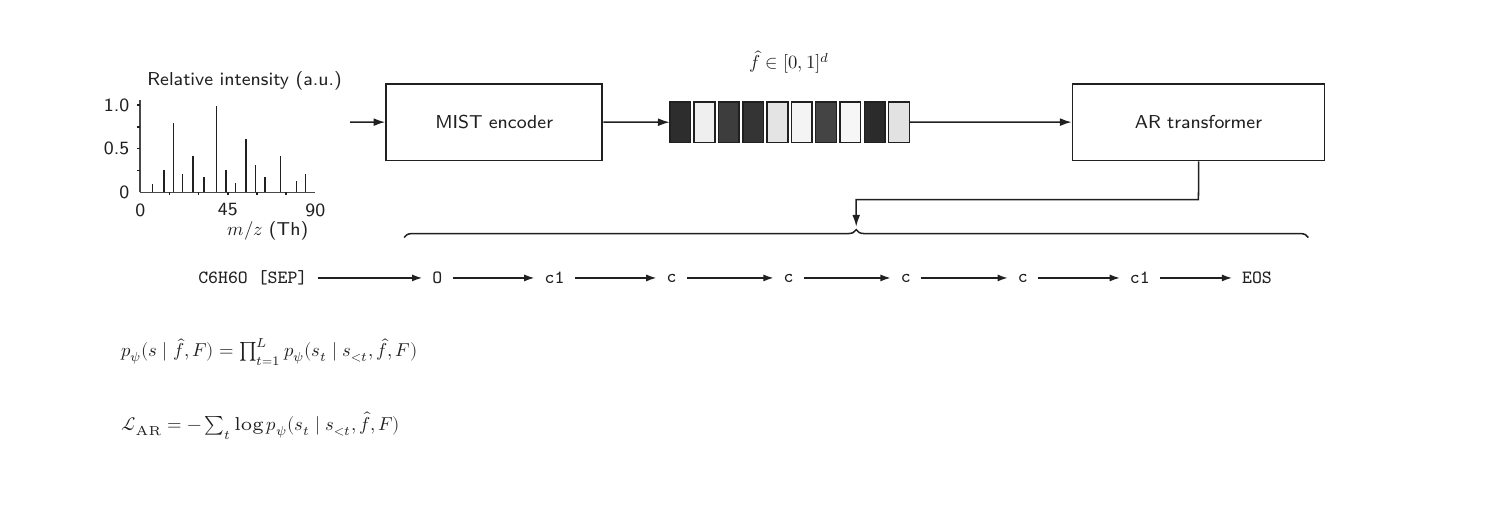
\begin{tikzpicture}[x=1cm,y=1cm,scale=1.14375,transform shape]
\spectrum{1.25}{5.02}{.54}
\node[box,minimum width=2.4cm,text width=2.1cm,minimum height=.85cm,inner sep=4pt] (arencoder) at (5.18,5.80) {MIST encoder};
\draw[arr] (3.58,5.80)--(arencoder.west);
% Probability-valued fingerprint dimensions, shown as a vector rather than a process box.
\foreach \i/\shade in {0/94,1/7,2/87,3/91,4/12,5/5,6/84,7/4,8/95,9/13}{\draw[draw=ink,line width=.55pt,fill=ink!\shade] (7.13+\i*.27,5.575) rectangle +(.23,.45);}
\node[small,inner sep=0] at (8.46,6.47) {$\hat f\in[0,1]^d$};
\node[box,minimum width=2.8cm,text width=2.5cm,minimum height=.85cm,inner sep=4pt] (ardecoder) at (13.0,5.80) {AR transformer};
\draw[arr] (arencoder.east)--(7.13,5.80);\draw[arr] (9.79,5.80)--(ardecoder.west);
% The decoder emits the complete token sequence; a brace attaches the output arrow to it.
\node[inner sep=0,font=\figurefont] (arprefix) at (2.50,4.07) {\texttt{C6H6O [SEP]}};
\foreach \i/\t in {0/O,1/c1,2/c,3/c,4/c,5/c,6/c1,7/EOS}{\node[inner sep=0,font=\figurefont] (artoken\i) at (4.55+\i*1.30,4.07) {\texttt{\t}};}
\draw[thinarr,shorten <=.12cm,shorten >=.12cm] (arprefix.east)--(artoken0.west);
\foreach \i/\j in {0/1,1/2,2/3,3/4,4/5,5/6,6/7}{\draw[thinarr,shorten <=.12cm,shorten >=.12cm] (artoken\i.east)--(artoken\j.west);}
\draw[ink,line width=.55pt,decorate,decoration={brace,amplitude=.10cm}] (4.18,4.52)--(14.22,4.52);
\draw[arr] (ardecoder.south)--(13.0,4.94)--(9.20,4.94)--(9.20,4.64);
\node[anchor=west,inner sep=0,font=\figurefont] at (1.03,3.25) {$\textstyle p_\psi(s\mid\hat f,F)=\prod_{t=1}^{L}p_\psi(s_t\mid s_{<t},\hat f,F)$};
\node[anchor=west,inner sep=0,font=\figurefont] at (1.03,2.43) {$\textstyle\mathcal L_{\rm AR}=-\sum\nolimits_t\log p_\psi(s_t\mid s_{<t},\hat f,F)$};
% Fixed canvas: 183 x 60.046875 mm. No clipping: overflow is audited.
\pgfresetboundingbox
\path[use as bounding box] (0,1.6) rectangle (16,6.85);
\end{tikzpicture}
\end{document}
